\chapter{Sprint 0}
\section{Introduction}
\label{sec:intro_sprint0}

Ce chapitre présente le Sprint 0, la phase initiale du projet visant à développer un système de collecte de données en temps réel et de gestion des alertes pour les appareils médicaux en salle de réveil. Le Sprint 0 pose les bases en identifiant les acteurs clés, en capturant les besoins fonctionnels et non fonctionnels, et en définissant la méthodologie Scrum qui guidera les phases de développement ultérieures. Cette phase garantit l'alignement avec les objectifs du projet d'améliorer la surveillance post-opératoire grâce à la collecte automatisée de données et aux alertes en temps réel, comme décrit dans les chapitres \ref{chap:introduction} et \ref{chap:architecture}.

\section{Capture des besoins}
\subsection{Identification des acteurs}
\label{subsec:acteurs}

Le système interagit avec plusieurs acteurs clés, chacun ayant des rôles distincts essentiels à son fonctionnement. Ces acteurs, résumés dans le tableau \ref{tab:acteurs}, sont alignés sur le contexte médical décrit dans le chapitre \ref{chap:introduction} et les composants architecturaux du chapitre \ref{chap:architecture}.

\begin{table}[h]
\centering
\caption{Acteurs du système et leurs rôles}
\label{tab:acteurs}
\begin{tabular}{|p{3cm}|p{9cm}|}
\hline
\textbf{Acteur} & \textbf{Description} \\
\hline
Médecin & Consulte les données des patients, reçoit les alertes critiques et valide les actions nécessaires. \\
\hline
Infirmier(ère) & Surveille les patients, reçoit les alertes en fonction de ses horaires et prend des mesures immédiates. \\
\hline
Administrateur du Système & Gère les utilisateurs, configure les seuils d'alerte et assure le bon fonctionnement du système. \\
\hline
Moniteur de Signes Vitaux & Source de données des signes vitaux, transmises via API ou OCR basé sur caméra. \\
\hline
Caméra & Capture les écrans des moniteurs pour l'extraction des données via YOLO et OCR. \\
\hline
\end{tabular}
\end{table}

\subsection{Besoins fonctionnels et non fonctionnels}
\label{subsec:besoins}

Les besoins fonctionnels et non fonctionnels reflètent les objectifs du système d'automatiser la collecte de données, d'améliorer la gestion des alertes et de garantir l'évolutivité et la conformité, comme introduit dans le chapitre \ref{chap:introduction}.

\textbf{Besoins Fonctionnels :}
\begin{itemize}
    \item \textbf{Collecte des données :} Collecte en temps réel des données des moniteurs de signes vitaux (par exemple, Mindray, Edan) à l'aide de caméras et d'OCR, comme détaillé dans la section \ref{sec:architecture_globale}.
    \item \textbf{Détection et reconnaissance des valeurs vitales :} Extraction des signes vitaux (fréquence cardiaque, pression artérielle, SpO2) en utilisant YOLOv8 pour la détection des régions et Tesseract OCR pour l'extraction de texte \cite{redmon_yolo_2023, tesseract_ocr_2023}.
    \item \textbf{Génération et gestion des alertes :} Déclenchement des alertes en fonction de seuils prédéfinis, configurables dynamiquement.
    \item \textbf{Afficher les données :} Interfaces web (React) et mobile (Flutter) pour la visualisation des données en temps réel et la gestion des alertes.
    \item \textbf{Authentification et gestion des utilisateurs :} Contrôle d'accès basé sur les rôles pour les médecins, infirmiers et administrateurs à l'aide de Sanctum de Laravel \cite{laravel_docs_2023}.
    \item \textbf{Notifications :} Notifications push en temps réel via Firebase Cloud Messaging (FCM), e-mails et SMS \cite{firebase_fcm_2023}.
    \item \textbf{Stockage et historique des données :} Stockage des mesures et des alertes dans une base de données MySQL pour analyse et suivi \cite{mysql_docs_2023}.
\end{itemize}

\textbf{Besoins Non Fonctionnels :}
\begin{itemize}
    \item \textbf{Disponibilité :} Accessibilité du système 24/7 avec un temps d'arrêt minimal (< 0,01 \%).
    \item \textbf{Sécurité :} Chiffrement des données (AES-256) et authentification sécurisée pour protéger les données des patients, conforme aux réglementations médicales (par exemple, RGPD, HIPAA).
    \item \textbf{Interopérabilité :} Compatibilité avec divers modèles de moniteurs (Mindray, Edan).
    \item \textbf{Évolutivité :} Capacité à gérer une augmentation du nombre de patients et d'appareils (jusqu'à 1000 patients simultanés).
    \item \textbf{Temps de réponse :} Traitement instantané des alertes pour les situations critiques (< 2 secondes).
    \item \textbf{Conformité :} Respect des réglementations de protection des données médicales.
\end{itemize}

\subsection{Diagramme des cas d'utilisation global}
\label{subsec:cas_utilisation}

Le diagramme global des cas d'utilisation (Figure \ref{fig:cas_utilisation}) illustre les interactions entre les acteurs et le système, y compris la consultation des données, la réception des alertes et l'administration du système. Des prototypes pour les interfaces web et mobile ont été développés pour visualiser les données et gérer les alertes, garantissant l'alignement avec les besoins des utilisateurs identifiés dans la section \ref{subsec:acteurs}.

\begin{figure}[h]
\centering
\caption{Diagramme des cas d'utilisation global}
\label{fig:cas_utilisation}
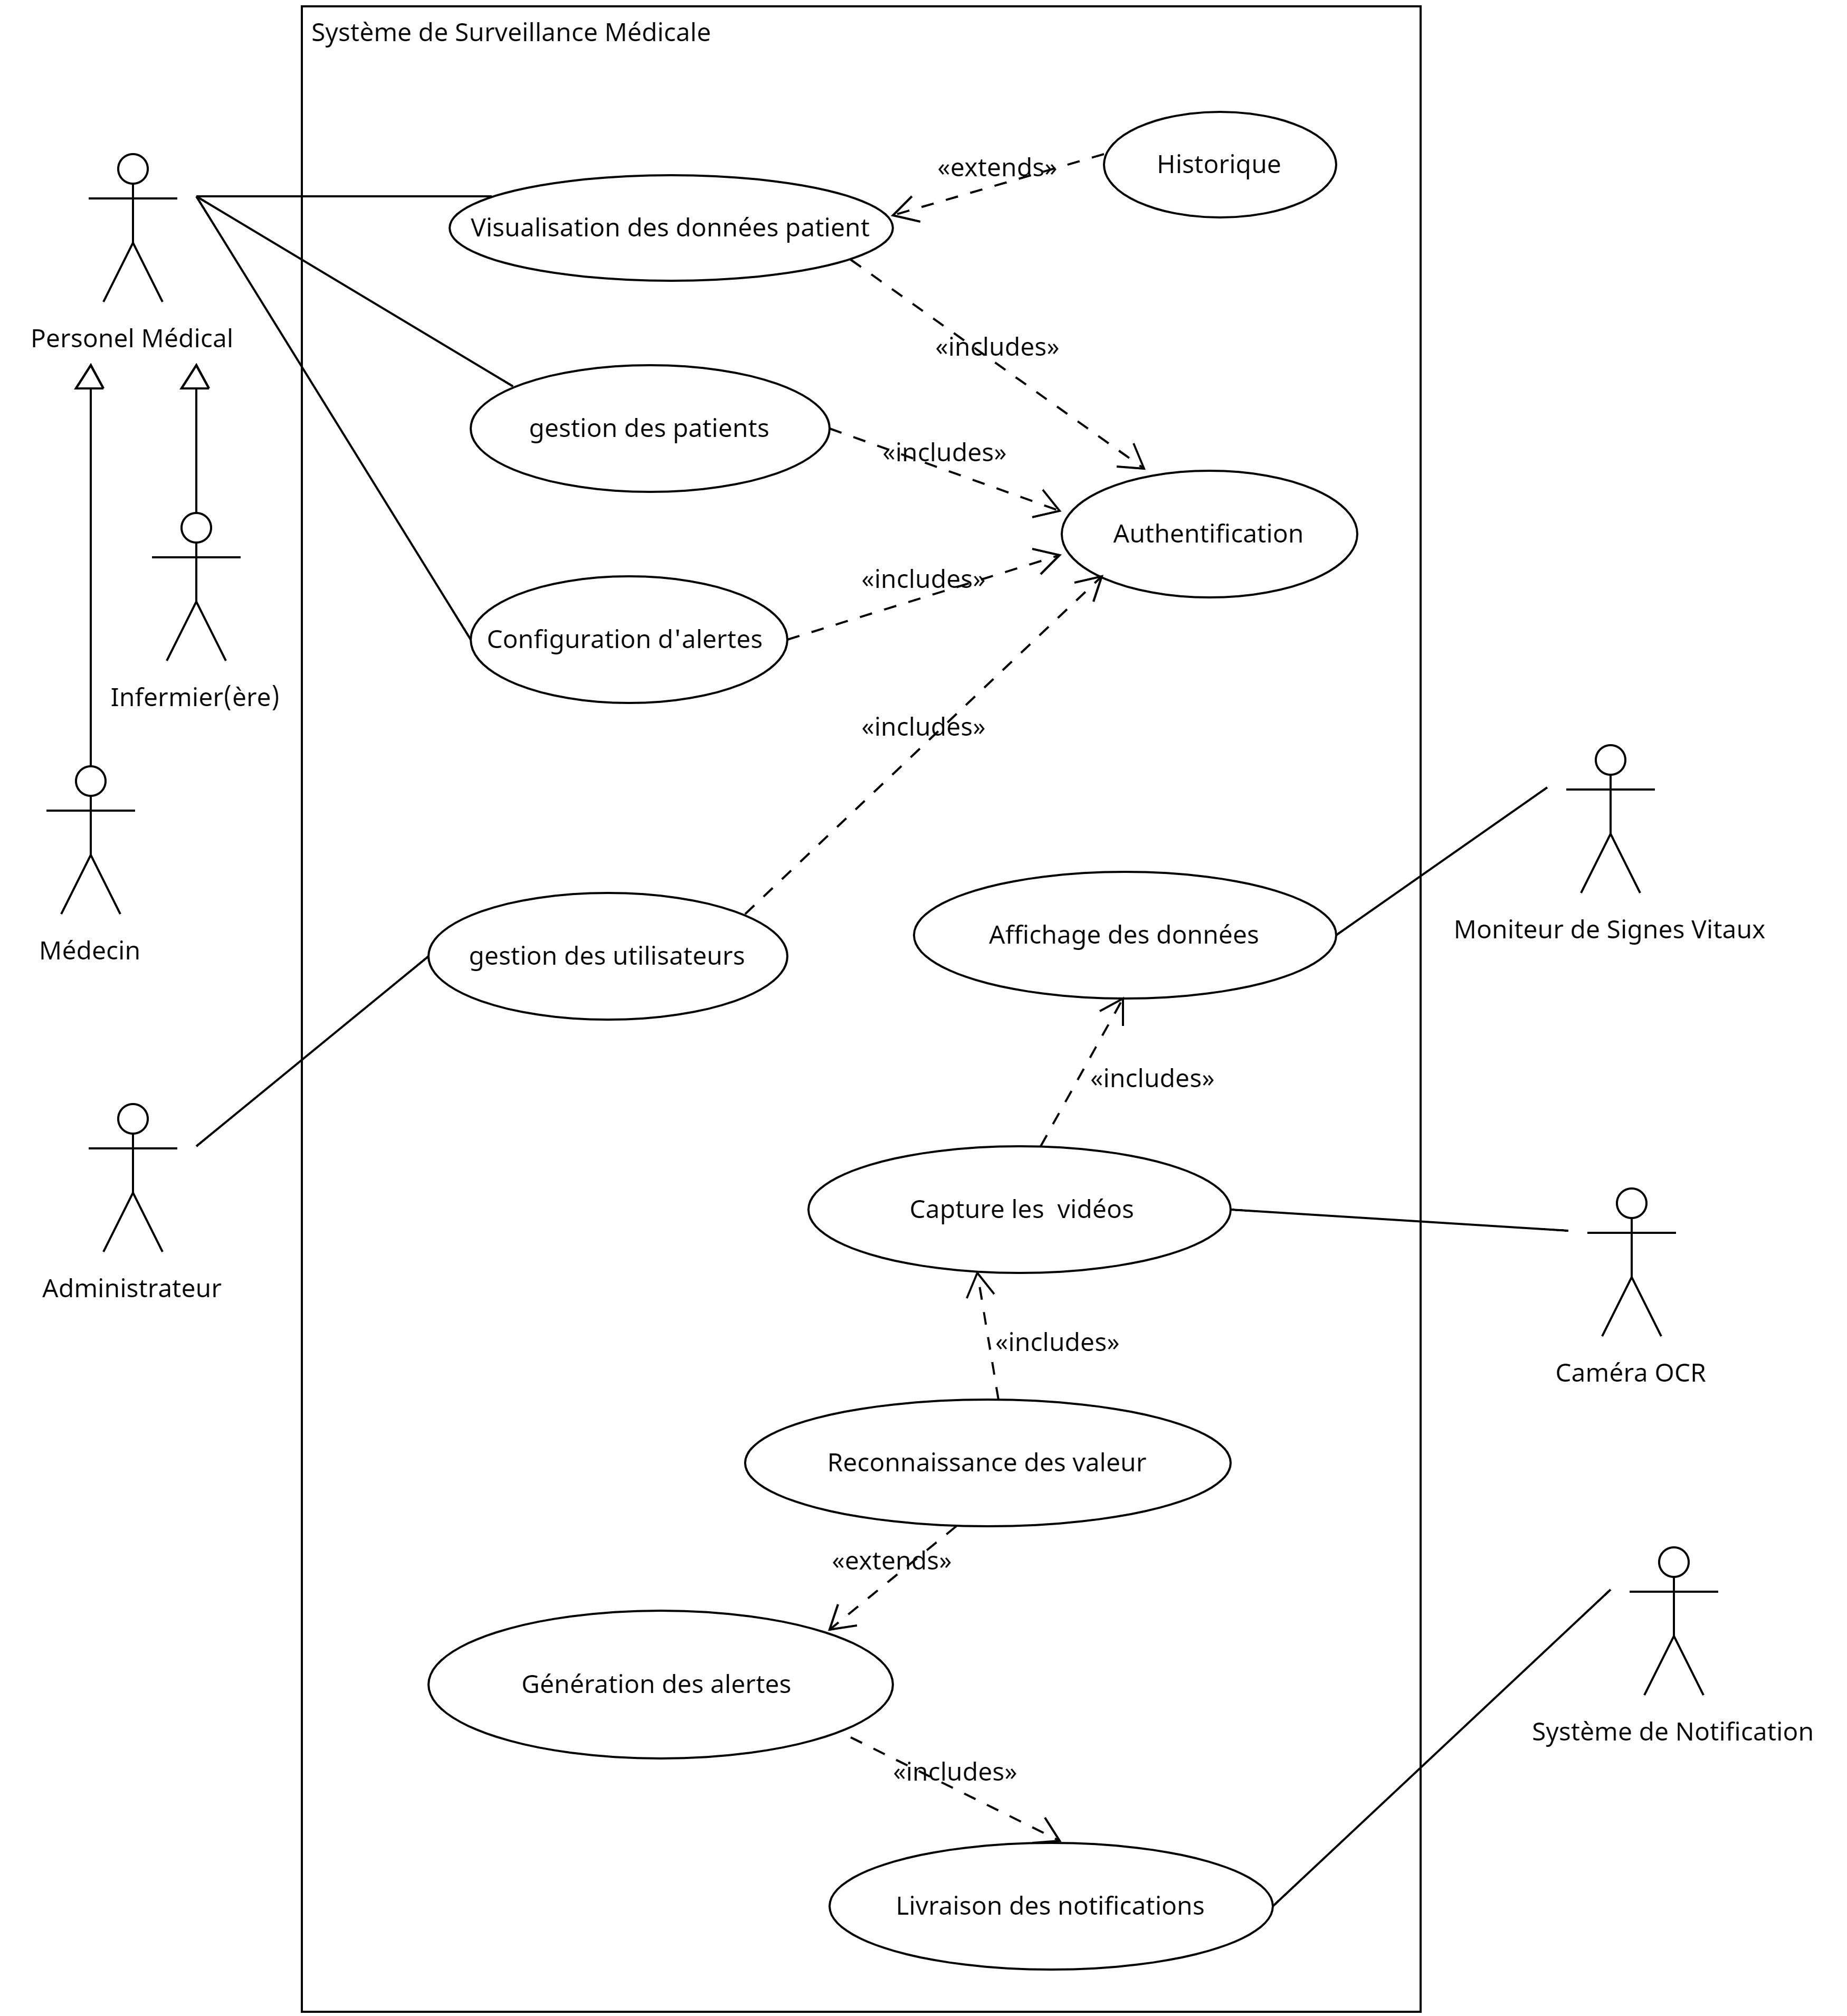
\includegraphics[width=0.8\textwidth]{chapter4/sections/diagrams/use_case.png}
\end{figure}

\section{Pilotage du projet avec Scrum}
\label{sec:gestion_scrum}

Le projet adopte la méthodologie Scrum, comme justifié dans le chapitre \ref{chap:methodologie}, pour garantir un développement itératif et une collaboration avec
les parties prenantes. Cette section détaille les rôles Scrum, l'organisation du backlog et la planification des sprints pour le Sprint 0.

\subsection{Acteurs Scrum et Missions}
\label{subsec:roles_scrum}

Les rôles Scrum et leurs responsabilités sont définis dans le tableau \ref{tab:roles_scrum}, assurant l'alignement avec l'approche collaborative décrite dans la section \ref{sec:roles_scrum}.

\begin{table}[h]
\centering
\caption{Acteurs du projet Scrum}
\label{tab:roles_scrum}
\begin{tabular}{|p{3cm}|p{7cm}|p{3cm}|}
\hline
\textbf{Rôle} & \textbf{Mission} & \textbf{Acteur} \\
\hline
Product Owner & Définir et prioriser les fonctionnalités du produit (Product Backlog), valider les livrables. & Pr Ammeri Charfeddine \\
\hline
Équipe de Développement & Concevoir, développer et tester les fonctionnalités, assurer la qualité du code. & Zaibi Racha \\
\hline
Scrum Master & Faciliter les événements Scrum, supprimer les obstacles, assurer l'adhésion à Scrum. & Ouni Ghada \\
\hline
\end{tabular}
\end{table}

\subsection{Organisation du Backlog}
\label{subsec:backlog}

Le Product Backlog, géré via ClickUp \cite{clickup_docs_2025}, est organisé en utilisant la méthode de priorisation MoSCoW pour s'aligner sur les objectifs du projet. Chaque fonctionnalité est formulée comme une User Story pour garantir un développement centré sur l'utilisateur. Le tableau \ref{tab:backlog} liste les tâches priorisées, avec des références à l'architecture technique du chapitre \ref{chap:architecture}.

\begin{table}[h]
\centering
\caption{Backlog du Projet avec Priorités MoSCoW}
\label{tab:backlog}
\begin{tabular}{|p{1.5cm}|p{8cm}|p{1.5cm}|}
\hline
\textbf{ID} & \textbf{Tâche} & \textbf{Priorité} \\
\hline
M-01 & Détection et reconnaissance des valeurs vitales via YOLO et OCR pour les moniteurs. & M \\
\hline
M-02 & Génération et gestion des alertes en fonction des seuils prédéfinis. & M \\
\hline
M-03 & Envoi d'alertes via notifications push (FCM) et e-mail. & M \\
\hline
M-04 & Interface web (React) et mobile (Flutter) pour visualiser les données et gérer les alertes. & M \\
\hline
M-05 & Authentification et gestion des utilisateurs (médecins, infirmiers, administrateurs). & M \\
\hline
M-06 & Stockage et historique des données dans MySQL. & M \\
\hline
M-07 & Conformité aux réglementations médicales (sécurité des données). & M \\
\hline
S-02 & Configuration des seuils d'alerte personnalisés par patient. & S \\
\hline
S-03 & Gestion des horaires de filtrage des alertes pour le personnel médical. & S \\
\hline
S-04 & Interface d'administration pour configurer les seuils et gérer les utilisateurs. & S \\
\hline
S-05 & Optimisation des notifications push pour faible latence. & S \\
\hline
C-04 & Support multilingue pour l'interface utilisateur. & C \\
\hline
C-05 & Gestion des alertes par priorité (critique, moyen, faible). & C \\
\hline
C-06 & Historique des alertes avec filtrage par date, patient, ou type d'alerte. & C \\
\hline
W-03 & Analyse avancée des données avec intelligence artificielle pour le diagnostic. & W \\
\hline
\end{tabular}
\end{table}

\textbf{Clé des Priorités MoSCoW :}
\begin{itemize}
    \item \textbf{M (Must) :} Tâches critiques nécessaires au fonctionnement du système.
    \item \textbf{S (Should) :} Tâches importantes apportant une valeur significative mais non essentielles pour la première version.
    \item \textbf{C (Could) :} Fonctionnalités optionnelles pouvant être ajoutées si le temps et les ressources le permettent.
    \item \textbf{W (Won't Have) :} Tâches hors du périmètre de la phase actuelle du projet.
\end{itemize}

\subsection{Planification des sprints}
\label{subsec:planification_sprints}

Le projet est divisé en trois sprints, chacun d'une durée de trois semaines, comme illustré dans la figure \ref{fig:processus_scrum} (voir section \ref{sec:presentation_scrum}). La réunion de planification du Sprint 0 a identifié les tâches et les livrables, en alignement avec les besoins des parties prenantes et les composants architecturaux (par exemple, YOLO, OCR, FCM) décrits dans le chapitre \ref{chap:architecture}.

\textbf{Sprint 1 : Création du dataset et mise en place du pipeline OCR}
\begin{itemize}
    \item \textbf{Objectif :} Développer un pipeline OCR basé sur YOLO en utilisant des images pré-capturées des moniteurs Mindray et Edan.
    \item \textbf{Livrables :}
        \begin{itemize}
            \item Dataset annoté (images des moniteurs Mindray et Edan avec signes vitaux).
            \item Modèle YOLOv8 entraîné pour détecter les zones des signes vitaux (par exemple, fréquence cardiaque, SpO2, pression artérielle).
            \item Pipeline OCR (YOLOv8 + Tesseract) pour extraire les valeurs des zones détectées.
        \end{itemize}
    \item \textbf{Durée :} 3 semaines.
    \item \textbf{Tâches principales :}
        \begin{itemize}
            \item Capturer et annoter les images des moniteurs (boîtes englobantes des signes vitaux) avec LabelImg \cite{labelimg_2023}.
            \item Entraîner le modèle YOLOv8 sur le dataset annoté.
            \item Intégrer OpenCV et Tesseract OCR pour extraire le texte des régions détectées \cite{opencv_2023, tesseract_ocr_2023}.
            \item Configurer les caméras IP (1080p, montage fixe) pour la capture des images.
        \end{itemize}
    \item \textbf{Critères d'acceptation :}
        \begin{itemize}
            \item YOLOv8 atteint un mAP $\geq 90\%$ sur le jeu de test (validé sur 100 images).
            \item L'OCR extrait les valeurs avec une précision $\geq 95\%$ (comparée à 20 vérifications manuelles).
            \item Latence du pipeline OCR $< 1$ seconde par image dans 100\% des tests.
            \item Compatibilité avec les moniteurs Mindray et Edan, testée dans 5 scénarios.
        \end{itemize}
    \item \textbf{Risques :}
        \begin{itemize}
            \item Mauvais éclairage ou angles des images affectant la précision. \textbf{Solution :} Optimiser le prétraitement avec des filtres OpenCV (par exemple, ajustement de contraste).
            \item Taille insuffisante du dataset. \textbf{Solution :} Augmenter les données via des techniques d'augmentation (rotation, recadrage).
        \end{itemize}
\end{itemize}

\textbf{Sprint 2 : Système d'alerte et gestion du personnel}
\begin{itemize}
    \item \textbf{Objectif :} Mettre en place un système d'alertes en temps réel et de notifications basées sur les rôles des utilisateurs.
    \item \textbf{Livrables :}
        \begin{itemize}
            \item Moteur d'alerte basé sur des règles (seuils pour fréquence cardiaque, SpO2, pression artérielle).
            \item Système de notification basé sur les rôles (médecins, infirmiers).
            \item Intégration de Firebase Cloud Messaging (FCM) pour les alertes mobiles \cite{firebase_fcm_2023}.
        \end{itemize}
    \item \textbf{Durée :} 3 semaines.
    \item \textbf{Tâches principales :}
        \begin{itemize}
            \item Configurer les seuils d'alerte (par exemple, fréquence cardiaque $< 60$ ou $> 100$ bpm $\rightarrow$ ``Critique'' ; SpO2 $< 90\%$ $\rightarrow$ ``Critique'' ; pression artérielle systolique $> 180$ mmHg ou $< 90$ mmHg $\rightarrow$ ``Critique'').
            \item Associer les alertes aux rôles (par exemple, critiques $\rightarrow$ médecin ; avertissements $\rightarrow$ infirmier).
            \item Intégrer FCM pour l'envoi des notifications push sur Android et iOS.
            \item Développer un module de validation des données OCR pour garantir la fiabilité des alertes.
        \end{itemize}
    \item \textbf{Critères d'acceptation :}
        \begin{itemize}
            \item Alertes déclenchées en $< 2$ secondes après dépassement des seuils (testé sur 50 scénarios).
            \item Notifications envoyées aux bons rôles dans 100\% des cas (testé sur 20 utilisateurs).
            \item Précision des données validées $\geq 98\%$ (comparée à 20 vérifications manuelles).
            \item Notifications push reçues avec un taux de succès de 99\% sur Android et iOS.
        \end{itemize}
    \item \textbf{Dépendances :} Pipeline OCR fonctionnel du Sprint 1.
    \item \textbf{Risques :}
        \begin{itemize}
            \item Retards dans les notifications FCM. \textbf{Solution :} Tester avec des données simulées et optimiser la configuration FCM.
            \item Erreurs OCR affectant les alertes. \textbf{Solution :} Implémenter des tests unitaires supplémentaires pour l'OCR.
        \end{itemize}
\end{itemize}

\textbf{Sprint 3 : Interfaces utilisateur et tableau de bord des alertes}
\begin{itemize}
    \item \textbf{Objectif :} Développer des interfaces pour le suivi des alertes et les actions du personnel, avec stockage des données.
    \item \textbf{Livrables :}
        \begin{itemize}
            \item Tableau de bord web (React) pour les alertes en temps réel et les signes vitaux des patients.
            \item Application mobile (Flutter) pour la réception des alertes et l'accusé de réception par le personnel.
            \item Base de données MySQL pour enregistrer les alertes et les réponses du personnel \cite{mysql_docs_2023}.
        \end{itemize}
    \item \textbf{Durée :} 3 semaines.
    \item \textbf{Tâches principales :}
        \begin{itemize}
            \item Développer le tableau de bord React avec priorisation des alertes (critique, avertissement) \cite{react_docs_2023}.
            \item Créer l'application Flutter avec intégration FCM pour les accusés de réception \cite{flutter_docs_2023}.
            \item Configurer MySQL pour stocker les alertes, réponses, et historiques des signes vitaux.
            \item Implémenter des WebSockets pour les mises à jour en temps réel des interfaces.
        \end{itemize}
    \item \textbf{Critères d'acceptation :}
        \begin{itemize}
            \item Tableau de bord met à jour les signes vitaux et alertes toutes les 5 secondes (testé avec 10 utilisateurs simultanés).
            \item Application mobile reçoit et accuse réception des alertes avec un taux de succès de 99\% (testé sur 20 utilisateurs).
            \item Données stockées dans MySQL avec 100\% d'intégrité (validé sur 50 enregistrements).
            \item Ergonomie validée par 5 utilisateurs médicaux (aucun problème d'utilisabilité signalé).
        \end{itemize}
    \item \textbf{Dépendances :} Système d'alerte du Sprint 2.
    \item \textbf{Risques :}
        \begin{itemize}
            \item Latence de l'interface utilisateur. \textbf{Solution :} Optimiser les appels API avec WebSockets et effectuer des tests de charge.
            \item Complexité d'intégration des interfaces. \textbf{Solution :} Réaliser des prototypes préliminaires et des tests d'utilisabilité itératifs.
        \end{itemize}
\end{itemize}

\section{Environnement de travail}
\label{sec:environnement}

\subsection{Environnement matériel}
\label{subsec:materiel}

L'environnement matériel est aligné sur les exigences architecturales de la section \ref{sec:architecture_physique} :

\begin{itemize}
    \item \textbf{Caméras pour les moniteurs :} Caméras IP (1080p, montage fixe) pour capturer les écrans des moniteurs Mindray et Edan pour le traitement par YOLO et OCR.
    \item \textbf{Serveurs :} Serveurs locaux dédiés (Intel i5, 16 Go RAM, 500 Go SSD) pour le stockage, le traitement des données et la génération des alertes.
    \item \textbf{Réseau de communication :} LAN sécurisé avec accès Internet pour la transmission des données entre caméras, serveurs et applications.
    \item \textbf{Appareils mobiles :} Smartphones/tablettes (Android 8.0+ ou iOS 12+) pour les notifications et l'accès aux données en temps réel.
\end{itemize}

\subsection{Environnement de développement}
\label{subsec:dev_environnement}

L'environnement de développement utilise des outils cohérents avec les choix technologiques du chapitre \ref{chap:architecture} :

\begin{itemize}
    \item \textbf{Langages et Frameworks :}
        \begin{itemize}
            \item \textbf{Python 3.11.0 :} Pour le traitement des images (OpenCV, YOLOv8, Tesseract) et les services backend basés sur Flask \cite{opencv_2023, tesseract_ocr_2023}.
            \item \textbf{Laravel 11.44.2 :} Pour le développement backend, la gestion des utilisateurs et les services de notification \cite{laravel_docs_2023}.
            \item \textbf{React 18.3.1 :} Pour le tableau de bord web interactif \cite{react_docs_2023}.
            \item \textbf{Flutter 3.27.0 :} Pour l'application mobile multiplateforme \cite{flutter_docs_2023}.
        \end{itemize}
    \item \textbf{Bibliothèques et Outils :}
        \begin{itemize}
            \item \textbf{OpenCV :} Prétraitement des images et détection des régions d'intérêt \cite{opencv_2023}.
            \item \textbf{YOLOv8 :} Détection des régions pour les signes vitaux \cite{redmon_yolo_2023}.
            \item \textbf{Tesseract OCR :} Extraction de texte des images des moniteurs \cite{tesseract_ocr_2023}.
            \item \textbf{Firebase Cloud Messaging :} Notifications push en temps réel \cite{firebase_fcm_2023}.
            \item \textbf{LabelImg :} Annotation des images pour l'entraînement de YOLO \cite{labelimg_2023}.
            \item \textbf{Docker :} Conteneurisation des applications.
            \item \textbf{Git :} Contrôle de version via GitHub/GitLab \cite{pro_git_2014}.
        \end{itemize}
\end{itemize}

\subsection{Environnement logiciel}
\label{subsec:logiciel}

\begin{itemize}
    \item \textbf{Systèmes d'exploitation :}
        \begin{itemize}
            \item \textbf{Développement :} Windows 11 (16 Go RAM, Intel i5).
            \item \textbf{Mobile :} Android 14 ou iOS 12+.
        \end{itemize}
    \item \textbf{Base de données :} MySQL 9.1.0 pour le stockage relationnel avec conformité ACID \cite{mysql_docs_2023}.
    \item \textbf{Protocoles :}
        \begin{itemize}
            \item \textbf{API REST :} Communication sécurisée avec des tokens Bearer, documentée via Swagger.
            \item \textbf{WebSockets :} Notifications en temps réel.
        \end{itemize}
    \item \textbf{Outils :}
        \begin{itemize}
            \item \textbf{IDE :} Visual Studio Code, Android Studio.
            \item \textbf{Gestion des dépendances :} Composer (PHP), npm (JavaScript), pip (Python).
            \item \textbf{Tests :} Postman, Swagger pour tester les API.
        \end{itemize}
\end{itemize}

\section{Conclusion}
\label{sec:conclusion_sprint0}

Le Sprint 0 établit une base solide pour le projet en définissant les acteurs, les besoins et le cadre Scrum. Le Product Backlog priorisé, la planification détaillée des sprints et l'environnement de développement spécifié garantissent l'alignement avec les objectifs du projet de collecte de données en temps réel et de gestion des alertes. L'intégration de YOLO pour la détection des régions et d'OCR pour l'extraction des données, comme décrit dans le chapitre \ref{chap:architecture}, positionne le système pour un développement efficace dans les sprints suivants.

